\section{Selected optimized-target and double-excitation model}
The final development step replaces the auxiliary canonical-singles manifold
by a compact selected OO-CID space: the requested optimized, ground-orthogonal
ROKS singlets, their paired doubles, canonical frontier double excitations,
and the two exact four-spin singlets. Unoptimized auxiliary canonical singles
are omitted by excitation rank, using the same rule for every molecule.
This model-space choice was selected using thirteen exposed states. It is
an empirical design choice, not a proof that auxiliary singles always worsen
an orbital-optimized calculation. The common one-body reference averages
Fock Rayleigh quotients and qualified DFT orbital levels \emph{before} orbital
optimization, with weights $1/2,1/2$. This differs from averaging two separately
optimized parent energies. The exchange-response scale remains $\lambda=0.9$.
There is no orbital-gap scaling or fitted excitation offset.

Let $S_{IJ}$ be the CSF metric, $H^0_{IJ}$ the physical Slater--Condon
matrix element, and $d_I=E_I-H^0_{II}/S_{II}$. Away from the exact four-spin
block defined above, the effective matrix is
\begin{equation}
 H_{IJ}=H^0_{IJ}+\tfrac12 S_{IJ}(d_I+d_J).
\end{equation}
The native density functional supplies $E_I$ including spin polarization.
The excited-sector basis is projected orthogonal to the moving stationary
ground CSF $|0\rangle$, using
$|\widetilde I\rangle=|I\rangle-|0\rangle S_{0I}/S_{00}$.
We solve the resulting generalized eigenproblem and subtract the independently
stationary native ground energy. We differentiate this projector as well as
the CSF metric; using an unprojected full-SI root and shifting its energy is
not equivalent. The off-diagonal construction remains an approximate
state-interaction functional; it does not supply a universally balanced
multi-determinant ground-state functional.

The selected rule was frozen in commit \texttt{467a9e5} before evaluating
nitrosomethane and maleimide. All fifteen transitions satisfy the unchanged
aggregate MAE gate of 0.3 eV and individual error gate of 0.5 eV, with an MAE
of 0.220 eV and maximum absolute error 0.498 eV. The two post-freeze errors
are $-0.002$ and $+0.402$ eV, respectively, giving 0.202 eV MAE. These
molecules appeared in older campaigns: this is prospective validation of
the frozen candidate on historically exposed molecules, not a blind study.
Glyoxal is within only 0.002 eV of the individual gate; passing that gate
must not be interpreted as a universal correction to all $n\pi^*$ errors.
The same-reference, same-native-orbital TDA control gives 0.966 eV MAE over
these fifteen states. This control isolates the present kernel and is not
a claim to outperform every calibrated TDA or sTDA parameterization.

\begin{figure}[tbp]\centering
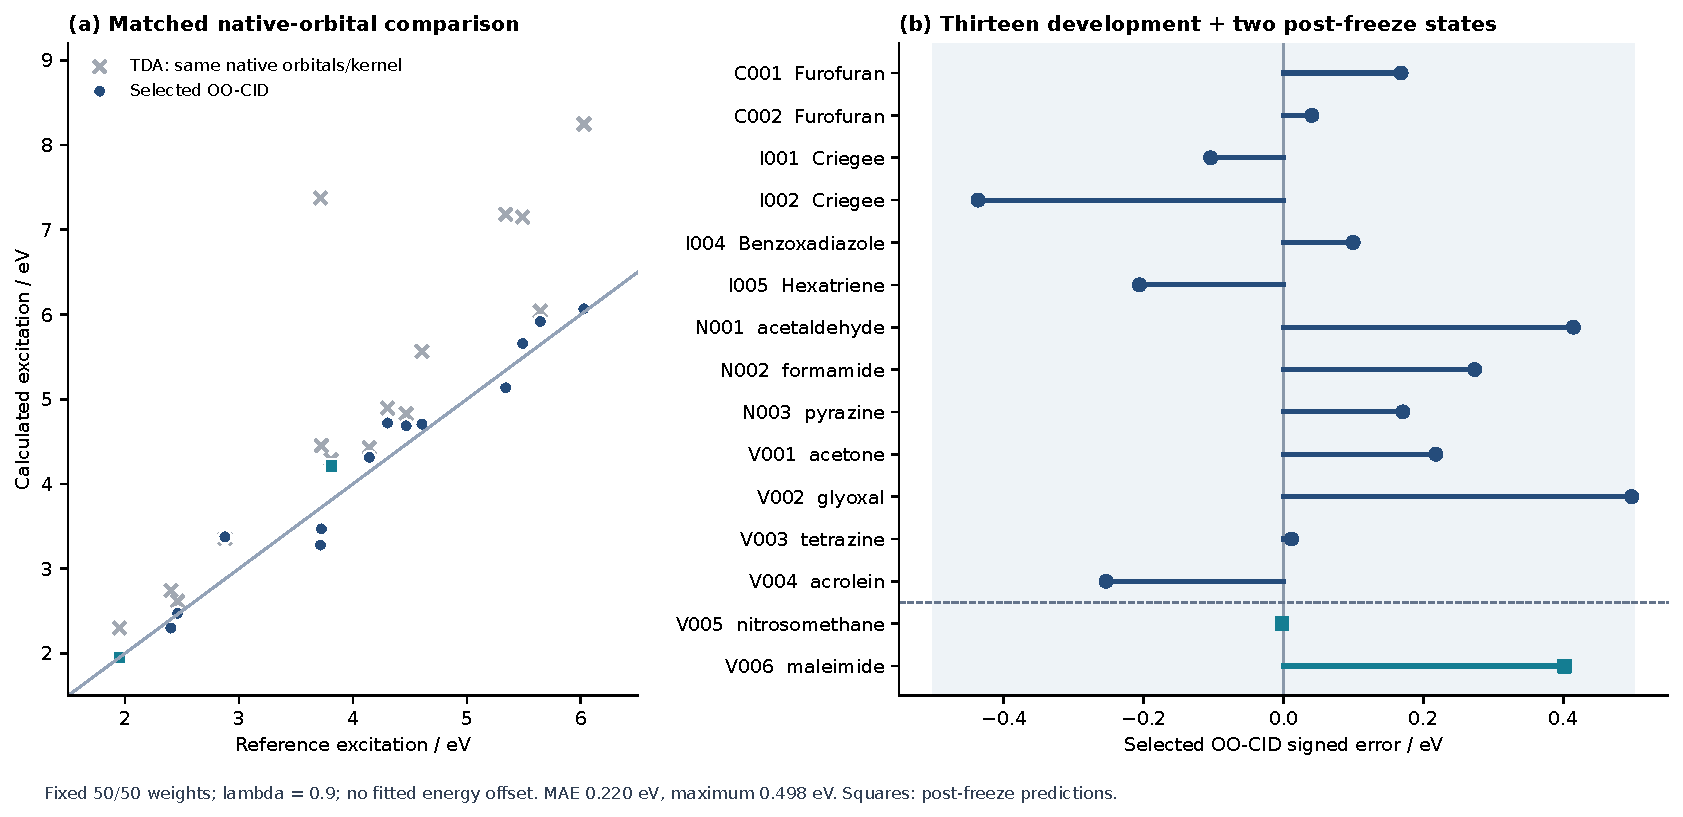
\includegraphics[width=\linewidth]{figures/selected_cid_validation.pdf}
\caption{Final selected OO-CID predictions. The shaded error interval is
$\pm0.5$ eV. Thirteen states informed model selection; squares identify the
two predictions made after the final candidate freeze. All controls use
native GFN2 spatial orbitals.}\end{figure}

The public class \texttt{PreparedNOSIModel} evaluates a portable, checksummed
MOUSE surface. LINK selects it with \texttt{nosi\_50\_50}. It uses native ground-program
Fock, energy and derivative machinery, constrained orbital optimization,
and a small CSF eigenproblem. It performs no TDA solve, DFT-backend import,
or fresh ground-state SCC calculation during evaluation. One-time DFT
reference preparation is still required. APOC follows coherent determinant
sums, preserving their phases and checking $\langle S^2\rangle=0$ using
$\|S_+\Psi\|^2$, rather than assigning spin purity to an $M_s=0$ determinant.
Only accepted LINK geometries advance an atomic, model-identified restart;
trial geometries leave that restart unchanged.

Complete analytic Hessians of the final selected model are verified for
Criegee (two states, 15 coordinates), glyoxal (one state, 18 coordinates),
and furofuran (two states, 36 coordinates). Independent reoptimized energy
checks at two displacement sizes and directions validate the first and
second derivatives; these finite differences are validation only. The largest Richardson-extrapolated
errors are $1.33\times10^{-10}$ Hartree/bohr for directional gradients and
$3.28\times10^{-7}$ Hartree/bohr$^2$ for directional curvatures. Both
first and second implicit KKT responses, the moving ground projector,
metric and generalized eigenvector response are retained. Physical operators
and auxiliary orbitals remain fixed in the co-rotating orthonormal AO frame;
this precisely defines an anchored PES, not a re-canonicalized model.
A fresh-process public-API Hessian reproduces the Criegee research matrices
within $9.1\times10^{-13}$ Hartree/bohr$^2$, taking 40.82 s with two BLAS
threads and 262 MiB peak RSS on MAC-STUDIO. Its energy-only evaluation takes
0.135 s. These timings exclude preparation and do not establish a vertical
speed advantage over TDA. The earlier 42.22 s phthalimide Hessian belongs
to the preceding production model, not this final selected candidate.

This completes a finite candidate test and automatic derivative integration.
It does not demonstrate an independent broad CT/Rydberg benchmark, final-model
excited minima and frequencies against coupled-cluster theory, or universal
chemical transferability. Those claims require additional evidence beyond
this compact valence-state set.
